\section{RQ8: Runtime and Lifecycle Value}
\label{sec:recovery}

NDC is implementation-independent search work; elapsed time is the deployment endpoint. We therefore report both without substituting one for the other.

\paragraph{Measured fixed-machine runtime.}
The S9-2 timing campaign pins one CPU, one search thread, and interleaves seven repetitions after 50 warmups over 24 builds per dataset. The original sub-millisecond per-cell CV criterion was rejected before policy gains were inspected; an amended action-block stability gate passes with exact native equivalence. The frozen source-slack candidate reduces wall time by 9.44 [9.04,9.77]\% on SIFT and 26.04 [25.62,26.44]\% on Arxiv. P95 ratios are 0.988 and 0.914, and minimum LOTO reductions are 9.42\% and 25.97\%. S9-3 and S9-4 independently retain positive fixed-machine wall-time reductions on fresh roles and builds.

\paragraph{Lifecycle accounting.}
For policy $\pi$ at horizon $N$,
\begin{equation}
 C_\pi(N)=C_{{\rm acquire},\pi}+N\bar c_\pi,
 \qquad N_{\rm BE}=\frac{\Delta C_{\rm acquire}}{\bar c_{\rm end}-\bar c_\pi}.
 \label{eq:breakeven}
\end{equation}
Cached history treats old profiles and truth as sunk; cold history charges their acquisition once per snapshot. Target selection, candidate and endpoint certification, and exact target truth are charged to recovery. At $N=10^6$, cold-history joint-error TCP saves about 490 million NDC on SIFT and 389 million on Arxiv; break-even is approximately 396,000 and 457,000 executions, compared with 129,000 and 148,000 under cached history. Four Arxiv fallback targets do not individually amortize positive recovery overhead.

\begin{table}[t]
\caption{Joint-error TCP break-even executions in thousands [95\% target-build interval]. ``No saving'' counts nonamortizing targets.}
\label{tab:economics}
\small\begin{tabular*}{\linewidth}{@{\extracolsep{\fill}}llrr@{}}\toprule
Dataset & History & Break-even, $10^3$ & No saving\\\midrule
\CostRows
\bottomrule\end{tabular*}
\end{table}

The post-seal target-certified Faiss ledger charges one 500-query target audit per target and reuses it across 23 source histories. Portfolio break-even is 66,914/17,018 executions under pairwise accounting and 3,019/755 under shared-target accounting for SIFT/Arxiv. These are NDC ledgers. Historical source acquisition and exact-truth/control wall time are unavailable and are not assigned zero. The measured S9 timing results establish serving latency reduction on one machine; they do not convert the NDC lifecycle model into a hardware-general monetary claim.

\begin{figure}[t]
\centering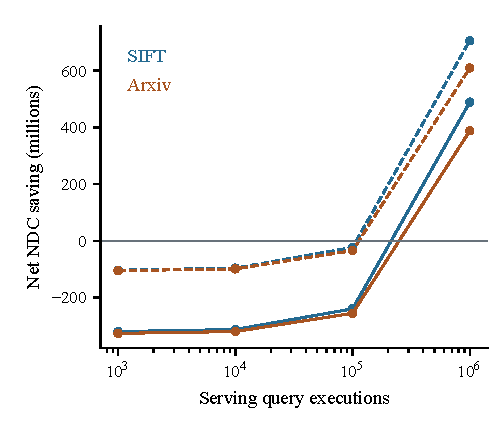
\includegraphics[width=\linewidth]{figures/cost.pdf}
\caption{Modeled joint-error TCP net distance saving versus serving horizon. Cold history crosses zero later than cached history; fallback targets remain in the average.}
\label{fig:cost}
\Description{Net distance savings become positive only after the acquisition cost is amortized over a sufficiently long serving horizon.}
\end{figure}
